% Options for packages loaded elsewhere
\PassOptionsToPackage{unicode}{hyperref}
\PassOptionsToPackage{hyphens}{url}
%
\documentclass[
]{book}
\usepackage{amsmath,amssymb}
\usepackage{lmodern}
\usepackage{ifxetex,ifluatex}
\ifnum 0\ifxetex 1\fi\ifluatex 1\fi=0 % if pdftex
  \usepackage[T1]{fontenc}
  \usepackage[utf8]{inputenc}
  \usepackage{textcomp} % provide euro and other symbols
\else % if luatex or xetex
  \usepackage{unicode-math}
  \defaultfontfeatures{Scale=MatchLowercase}
  \defaultfontfeatures[\rmfamily]{Ligatures=TeX,Scale=1}
\fi
% Use upquote if available, for straight quotes in verbatim environments
\IfFileExists{upquote.sty}{\usepackage{upquote}}{}
\IfFileExists{microtype.sty}{% use microtype if available
  \usepackage[]{microtype}
  \UseMicrotypeSet[protrusion]{basicmath} % disable protrusion for tt fonts
}{}
\makeatletter
\@ifundefined{KOMAClassName}{% if non-KOMA class
  \IfFileExists{parskip.sty}{%
    \usepackage{parskip}
  }{% else
    \setlength{\parindent}{0pt}
    \setlength{\parskip}{6pt plus 2pt minus 1pt}}
}{% if KOMA class
  \KOMAoptions{parskip=half}}
\makeatother
\usepackage{xcolor}
\IfFileExists{xurl.sty}{\usepackage{xurl}}{} % add URL line breaks if available
\IfFileExists{bookmark.sty}{\usepackage{bookmark}}{\usepackage{hyperref}}
\hypersetup{
  pdftitle={Tutoriais de Estatística},
  pdfauthor={Laboratório de Estatística Aplicada},
  hidelinks,
  pdfcreator={LaTeX via pandoc}}
\urlstyle{same} % disable monospaced font for URLs
\usepackage{color}
\usepackage{fancyvrb}
\newcommand{\VerbBar}{|}
\newcommand{\VERB}{\Verb[commandchars=\\\{\}]}
\DefineVerbatimEnvironment{Highlighting}{Verbatim}{commandchars=\\\{\}}
% Add ',fontsize=\small' for more characters per line
\usepackage{framed}
\definecolor{shadecolor}{RGB}{248,248,248}
\newenvironment{Shaded}{\begin{snugshade}}{\end{snugshade}}
\newcommand{\AlertTok}[1]{\textcolor[rgb]{0.94,0.16,0.16}{#1}}
\newcommand{\AnnotationTok}[1]{\textcolor[rgb]{0.56,0.35,0.01}{\textbf{\textit{#1}}}}
\newcommand{\AttributeTok}[1]{\textcolor[rgb]{0.77,0.63,0.00}{#1}}
\newcommand{\BaseNTok}[1]{\textcolor[rgb]{0.00,0.00,0.81}{#1}}
\newcommand{\BuiltInTok}[1]{#1}
\newcommand{\CharTok}[1]{\textcolor[rgb]{0.31,0.60,0.02}{#1}}
\newcommand{\CommentTok}[1]{\textcolor[rgb]{0.56,0.35,0.01}{\textit{#1}}}
\newcommand{\CommentVarTok}[1]{\textcolor[rgb]{0.56,0.35,0.01}{\textbf{\textit{#1}}}}
\newcommand{\ConstantTok}[1]{\textcolor[rgb]{0.00,0.00,0.00}{#1}}
\newcommand{\ControlFlowTok}[1]{\textcolor[rgb]{0.13,0.29,0.53}{\textbf{#1}}}
\newcommand{\DataTypeTok}[1]{\textcolor[rgb]{0.13,0.29,0.53}{#1}}
\newcommand{\DecValTok}[1]{\textcolor[rgb]{0.00,0.00,0.81}{#1}}
\newcommand{\DocumentationTok}[1]{\textcolor[rgb]{0.56,0.35,0.01}{\textbf{\textit{#1}}}}
\newcommand{\ErrorTok}[1]{\textcolor[rgb]{0.64,0.00,0.00}{\textbf{#1}}}
\newcommand{\ExtensionTok}[1]{#1}
\newcommand{\FloatTok}[1]{\textcolor[rgb]{0.00,0.00,0.81}{#1}}
\newcommand{\FunctionTok}[1]{\textcolor[rgb]{0.00,0.00,0.00}{#1}}
\newcommand{\ImportTok}[1]{#1}
\newcommand{\InformationTok}[1]{\textcolor[rgb]{0.56,0.35,0.01}{\textbf{\textit{#1}}}}
\newcommand{\KeywordTok}[1]{\textcolor[rgb]{0.13,0.29,0.53}{\textbf{#1}}}
\newcommand{\NormalTok}[1]{#1}
\newcommand{\OperatorTok}[1]{\textcolor[rgb]{0.81,0.36,0.00}{\textbf{#1}}}
\newcommand{\OtherTok}[1]{\textcolor[rgb]{0.56,0.35,0.01}{#1}}
\newcommand{\PreprocessorTok}[1]{\textcolor[rgb]{0.56,0.35,0.01}{\textit{#1}}}
\newcommand{\RegionMarkerTok}[1]{#1}
\newcommand{\SpecialCharTok}[1]{\textcolor[rgb]{0.00,0.00,0.00}{#1}}
\newcommand{\SpecialStringTok}[1]{\textcolor[rgb]{0.31,0.60,0.02}{#1}}
\newcommand{\StringTok}[1]{\textcolor[rgb]{0.31,0.60,0.02}{#1}}
\newcommand{\VariableTok}[1]{\textcolor[rgb]{0.00,0.00,0.00}{#1}}
\newcommand{\VerbatimStringTok}[1]{\textcolor[rgb]{0.31,0.60,0.02}{#1}}
\newcommand{\WarningTok}[1]{\textcolor[rgb]{0.56,0.35,0.01}{\textbf{\textit{#1}}}}
\usepackage{longtable,booktabs,array}
\usepackage{calc} % for calculating minipage widths
% Correct order of tables after \paragraph or \subparagraph
\usepackage{etoolbox}
\makeatletter
\patchcmd\longtable{\par}{\if@noskipsec\mbox{}\fi\par}{}{}
\makeatother
% Allow footnotes in longtable head/foot
\IfFileExists{footnotehyper.sty}{\usepackage{footnotehyper}}{\usepackage{footnote}}
\makesavenoteenv{longtable}
\usepackage{graphicx}
\makeatletter
\def\maxwidth{\ifdim\Gin@nat@width>\linewidth\linewidth\else\Gin@nat@width\fi}
\def\maxheight{\ifdim\Gin@nat@height>\textheight\textheight\else\Gin@nat@height\fi}
\makeatother
% Scale images if necessary, so that they will not overflow the page
% margins by default, and it is still possible to overwrite the defaults
% using explicit options in \includegraphics[width, height, ...]{}
\setkeys{Gin}{width=\maxwidth,height=\maxheight,keepaspectratio}
% Set default figure placement to htbp
\makeatletter
\def\fps@figure{htbp}
\makeatother
\setlength{\emergencystretch}{3em} % prevent overfull lines
\providecommand{\tightlist}{%
  \setlength{\itemsep}{0pt}\setlength{\parskip}{0pt}}
\setcounter{secnumdepth}{5}
\usepackage{booktabs}
\usepackage{amsthm}
\makeatletter
\def\thm@space@setup{%
  \thm@preskip=8pt plus 2pt minus 4pt
  \thm@postskip=\thm@preskip
}
\makeatother
\ifluatex
  \usepackage{selnolig}  % disable illegal ligatures
\fi
\usepackage[]{natbib}
\bibliographystyle{apalike}

\title{Tutoriais de Estatística}
\author{Laboratório de Estatística Aplicada}
\date{2021-02-09}

\begin{document}
\maketitle

{
\setcounter{tocdepth}{1}
\tableofcontents
}
\hypertarget{apresentacao}{%
\chapter*{Apresentação}\label{apresentacao}}
\addcontentsline{toc}{chapter}{Apresentação}

Essa página é uma iniciativa do \href{lea.estatistica.ccet.ufrn.br/}{Laboratório de Estatística Aplicada} do \href{https://sigaa.ufrn.br/sigaa/public/departamento/portal.jsf?id=47}{Departamento de Estatística da UFRN}. Nessa página é possível encontrar tutoriais em R para diversos métodos estatísticos no R.

Coordenação:

\begin{itemize}
\tightlist
\item
  \href{https://sigaa.ufrn.br/sigaa/public/docente/portal.jsf?siape=1218831}{Carla A. Vivacqua}
\item
  \href{https://marcusnunes.me}{Marcus Nunes}
\item
  Talita Barros
\end{itemize}

\hypertarget{estatisticadescritiva}{%
\chapter*{Estatística Descritiva}\label{estatisticadescritiva}}
\addcontentsline{toc}{chapter}{Estatística Descritiva}

Técnicas de visualização de dados.

\begin{Shaded}
\begin{Highlighting}[]
\FunctionTok{library}\NormalTok{(ggplot2)}
\FunctionTok{theme\_set}\NormalTok{(}\FunctionTok{theme\_bw}\NormalTok{())}

\FunctionTok{ggplot}\NormalTok{(mpg, }\FunctionTok{aes}\NormalTok{(}\AttributeTok{x =}\NormalTok{ displ, }\AttributeTok{y =}\NormalTok{ hwy)) }\SpecialCharTok{+}
  \FunctionTok{geom\_point}\NormalTok{() }\SpecialCharTok{+}
  \FunctionTok{facet\_wrap}\NormalTok{(}\SpecialCharTok{\textasciitilde{}}\NormalTok{ class, }\AttributeTok{ncol =} \DecValTok{2}\NormalTok{)}
\end{Highlighting}
\end{Shaded}

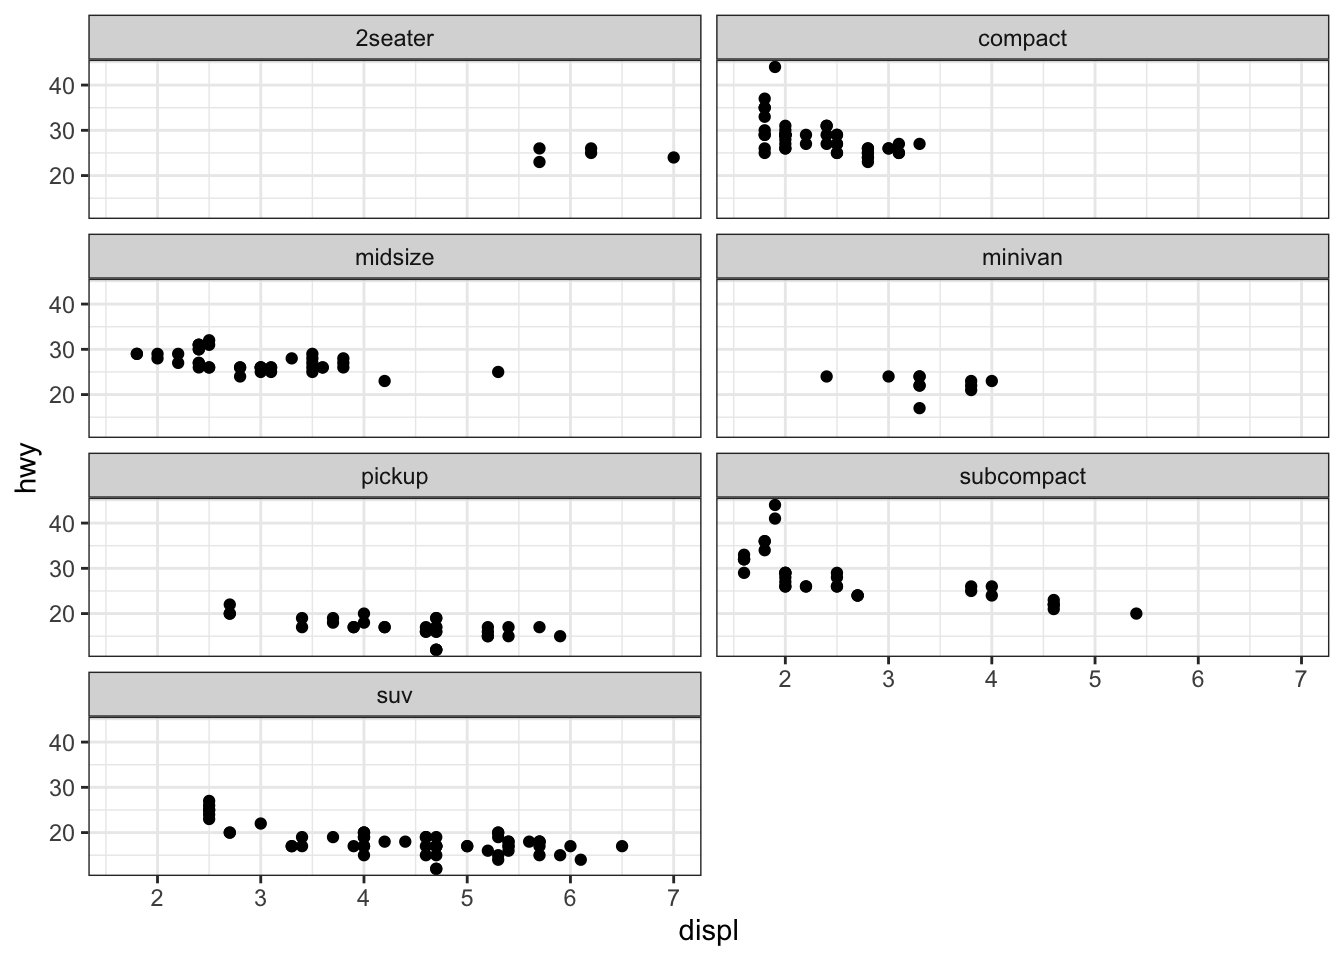
\includegraphics{bookdown-demo_files/figure-latex/estatisticadescritiva01-1.pdf}

\hypertarget{regressaolinearmultipla}{%
\chapter*{Regressao Linear Múltipla}\label{regressaolinearmultipla}}
\addcontentsline{toc}{chapter}{Regressao Linear Múltipla}

Alguma coisa sobre esse assunto.

\[y_i = \beta_0 + \beta_1x_{1i} + \cdots + \beta_px_{pi} + \varepsilon_i\]

\begin{Shaded}
\begin{Highlighting}[]
\NormalTok{ajuste }\OtherTok{\textless{}{-}} \FunctionTok{lm}\NormalTok{(Petal.Width }\SpecialCharTok{\textasciitilde{}}\NormalTok{ Petal.Length }\SpecialCharTok{+}\NormalTok{ Sepal.Width }\SpecialCharTok{+}\NormalTok{ Sepal.Length, }
             \AttributeTok{data =}\NormalTok{ iris)}
\FunctionTok{summary}\NormalTok{(ajuste)}
\end{Highlighting}
\end{Shaded}

\begin{verbatim}
## 
## Call:
## lm(formula = Petal.Width ~ Petal.Length + Sepal.Width + Sepal.Length, 
##     data = iris)
## 
## Residuals:
##      Min       1Q   Median       3Q      Max 
## -0.60959 -0.10134 -0.01089  0.09825  0.60685 
## 
## Coefficients:
##              Estimate Std. Error t value Pr(>|t|)    
## (Intercept)  -0.24031    0.17837  -1.347     0.18    
## Petal.Length  0.52408    0.02449  21.399  < 2e-16 ***
## Sepal.Width   0.22283    0.04894   4.553 1.10e-05 ***
## Sepal.Length -0.20727    0.04751  -4.363 2.41e-05 ***
## ---
## Signif. codes:  0 '***' 0.001 '**' 0.01 '*' 0.05 '.' 0.1 ' ' 1
## 
## Residual standard error: 0.192 on 146 degrees of freedom
## Multiple R-squared:  0.9379, Adjusted R-squared:  0.9366 
## F-statistic: 734.4 on 3 and 146 DF,  p-value: < 2.2e-16
\end{verbatim}

\hypertarget{regressaologistica}{%
\chapter*{Regressão Logística}\label{regressaologistica}}
\addcontentsline{toc}{chapter}{Regressão Logística}

Texto sobre regressão logística.

\begin{Shaded}
\begin{Highlighting}[]
\NormalTok{mydata }\OtherTok{\textless{}{-}} \FunctionTok{read.csv}\NormalTok{(}\StringTok{"https://stats.idre.ucla.edu/stat/data/binary.csv"}\NormalTok{)}
\NormalTok{mydata}\SpecialCharTok{$}\NormalTok{rank }\OtherTok{\textless{}{-}} \FunctionTok{factor}\NormalTok{(mydata}\SpecialCharTok{$}\NormalTok{rank)}

\NormalTok{mylogit }\OtherTok{\textless{}{-}} \FunctionTok{glm}\NormalTok{(admit }\SpecialCharTok{\textasciitilde{}}\NormalTok{ gre, }
               \AttributeTok{data =}\NormalTok{ mydata, }
               \AttributeTok{family =} \StringTok{"binomial"}\NormalTok{)}

\FunctionTok{summary}\NormalTok{(mylogit)}
\end{Highlighting}
\end{Shaded}

\begin{verbatim}
## 
## Call:
## glm(formula = admit ~ gre, family = "binomial", data = mydata)
## 
## Deviance Residuals: 
##     Min       1Q   Median       3Q      Max  
## -1.1623  -0.9052  -0.7547   1.3486   1.9879  
## 
## Coefficients:
##              Estimate Std. Error z value Pr(>|z|)    
## (Intercept) -2.901344   0.606038  -4.787 1.69e-06 ***
## gre          0.003582   0.000986   3.633  0.00028 ***
## ---
## Signif. codes:  0 '***' 0.001 '**' 0.01 '*' 0.05 '.' 0.1 ' ' 1
## 
## (Dispersion parameter for binomial family taken to be 1)
## 
##     Null deviance: 499.98  on 399  degrees of freedom
## Residual deviance: 486.06  on 398  degrees of freedom
## AIC: 490.06
## 
## Number of Fisher Scoring iterations: 4
\end{verbatim}

\begin{Shaded}
\begin{Highlighting}[]
\FunctionTok{library}\NormalTok{(ggplot2)}
\FunctionTok{theme\_set}\NormalTok{(}\FunctionTok{theme\_bw}\NormalTok{())}

\FunctionTok{ggplot}\NormalTok{(mydata, }\FunctionTok{aes}\NormalTok{(}\AttributeTok{x =}\NormalTok{ gre, }\AttributeTok{y =}\NormalTok{ admit)) }\SpecialCharTok{+}
  \FunctionTok{geom\_point}\NormalTok{() }\SpecialCharTok{+} 
  \FunctionTok{geom\_smooth}\NormalTok{(}\AttributeTok{method =} \StringTok{"glm"}\NormalTok{)}
\end{Highlighting}
\end{Shaded}

\begin{verbatim}
## `geom_smooth()` using formula 'y ~ x'
\end{verbatim}

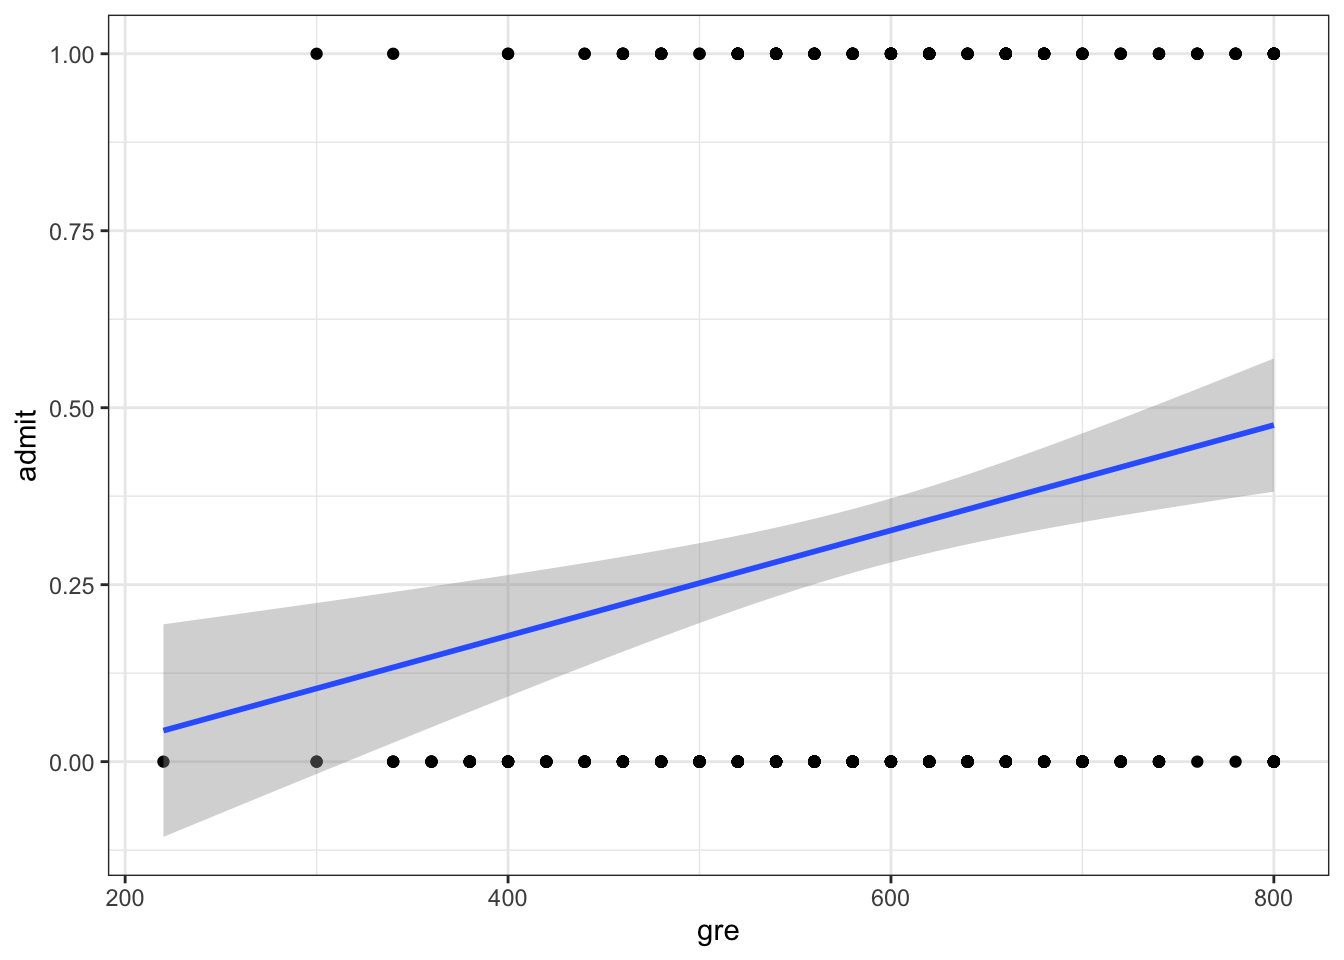
\includegraphics{bookdown-demo_files/figure-latex/regressaologistica01-1.pdf}

\hypertarget{estatisticanaoparametrica}{%
\chapter*{Estatística Não-Paramétrica}\label{estatisticanaoparametrica}}
\addcontentsline{toc}{chapter}{Estatística Não-Paramétrica}

Métodos usados quando não podemos assumir normalidade ou alguma outra distribuição de probabilidade em nossos dados.

\begin{Shaded}
\begin{Highlighting}[]
\NormalTok{x }\OtherTok{\textless{}{-}} \FunctionTok{c}\NormalTok{(}\FloatTok{2.9}\NormalTok{, }\FloatTok{3.0}\NormalTok{, }\FloatTok{2.5}\NormalTok{, }\FloatTok{2.6}\NormalTok{, }\FloatTok{3.2}\NormalTok{) }\CommentTok{\# normal subjects}
\NormalTok{y }\OtherTok{\textless{}{-}} \FunctionTok{c}\NormalTok{(}\FloatTok{3.8}\NormalTok{, }\FloatTok{2.7}\NormalTok{, }\FloatTok{4.0}\NormalTok{, }\FloatTok{2.4}\NormalTok{)      }\CommentTok{\# with obstructive airway disease}
\NormalTok{z }\OtherTok{\textless{}{-}} \FunctionTok{c}\NormalTok{(}\FloatTok{2.8}\NormalTok{, }\FloatTok{3.4}\NormalTok{, }\FloatTok{3.7}\NormalTok{, }\FloatTok{2.2}\NormalTok{, }\FloatTok{2.0}\NormalTok{) }\CommentTok{\# with asbestosis}

\NormalTok{dados }\OtherTok{\textless{}{-}} \FunctionTok{data.frame}\NormalTok{(}\AttributeTok{eficiencia =} \FunctionTok{c}\NormalTok{(x, y, z),}
                    \AttributeTok{grupo =} \FunctionTok{c}\NormalTok{(}\FunctionTok{rep}\NormalTok{(}\StringTok{"normal"}\NormalTok{, }\FunctionTok{length}\NormalTok{(x)),}
                              \FunctionTok{rep}\NormalTok{(}\StringTok{"obstrusivo"}\NormalTok{, }\FunctionTok{length}\NormalTok{(y)),}
                              \FunctionTok{rep}\NormalTok{(}\StringTok{"abestose"}\NormalTok{, }\FunctionTok{length}\NormalTok{(z)))}
\NormalTok{                    )}

\FunctionTok{kruskal.test}\NormalTok{(eficiencia }\SpecialCharTok{\textasciitilde{}}\NormalTok{ grupo,}
             \AttributeTok{data =}\NormalTok{ dados)}
\end{Highlighting}
\end{Shaded}

\begin{verbatim}
## 
##  Kruskal-Wallis rank sum test
## 
## data:  eficiencia by grupo
## Kruskal-Wallis chi-squared = 0.77143, df = 2, p-value = 0.68
\end{verbatim}

\begin{Shaded}
\begin{Highlighting}[]
\FunctionTok{library}\NormalTok{(ggplot2)}
\FunctionTok{theme\_set}\NormalTok{(}\FunctionTok{theme\_bw}\NormalTok{())}
\FunctionTok{library}\NormalTok{(reshape2)}

\FunctionTok{ggplot}\NormalTok{(dados, }\FunctionTok{aes}\NormalTok{(}\AttributeTok{x =}\NormalTok{ grupo, }\AttributeTok{y =}\NormalTok{ eficiencia)) }\SpecialCharTok{+}
  \FunctionTok{geom\_boxplot}\NormalTok{()}
\end{Highlighting}
\end{Shaded}

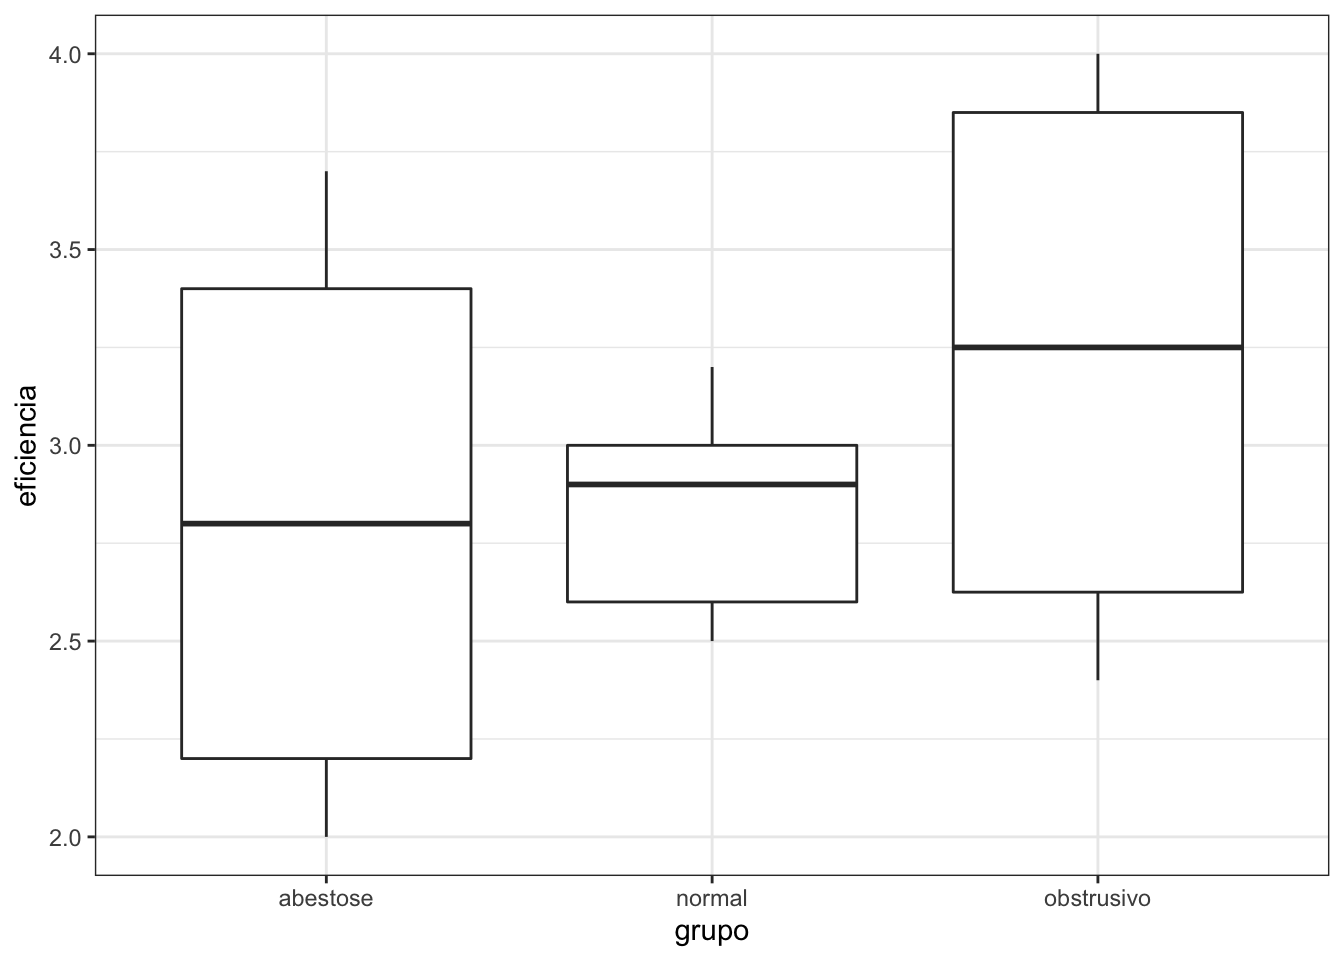
\includegraphics{bookdown-demo_files/figure-latex/estatisticanaoparametrica01-1.pdf}

  \bibliography{book.bib,packages.bib}

\end{document}
